\documentclass[tikz, border=5pt]{standalone}
\usetikzlibrary{arrows.meta, shapes, positioning, decorations.pathmorphing}

\tikzset{
  spring/.style = {
    decoration = {aspect=0.3, segment length=3mm, amplitude=3mm, coil},
    decorate
  }
}

\begin{document}

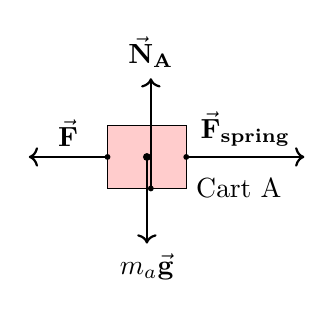
\begin{tikzpicture}

  % Cart A
  \draw[fill=red!20] (0,0) rectangle (1,0.8);
  \node [below, right] at (1,0) {Cart A};

  % Force F
  \draw[<-, thick] (-1,0.4) -- (0,0.4) node[midway, above] {\( \vec{\mathbf{F}} \)};
  \node[circle, fill, inner sep=0.75pt] at (0,0.4) {};

  % Spring Force
  \draw[->, thick] (1,0.4) -- (2.5,0.4) node[midway, above] {\( \mathbf{\vec{F}_{spring}} \)};
  \node[circle, fill, inner sep=0.75pt] at (1,0.4) {};

  % Normal reaction
  \draw[->, thick] (0.55,0) -- (0.55,1.4) node[above] {\( \mathbf{\vec{N}_A} \)};
  \node[circle, fill, inner sep=0.75pt] at (0.55,0) {};

  % Gravity
  \draw[->, thick] (0.5,0.4) -- (0.5,-0.7) node[below] {\( m_{a}\vec{\mathbf{g}} \)};
  \node[circle, fill, inner sep=1pt] at (0.5,0.4) {};

\end{tikzpicture}

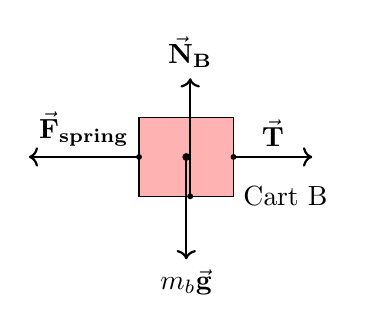
\begin{tikzpicture}

  % Cart B
  \draw[fill=red!30] (0,0) rectangle (1.2,1);
  \node [below, right] at (1.2,0) {Cart B};

  % Force T
  \draw[->, thick] (1.2,0.5) -- (2.2,0.5) node[midway, above] {\( \vec{\mathbf{T}} \)};
  \node[circle, fill, inner sep=0.75pt] at (1.2,0.5) {};

  % Spring Force
  \draw[<-, thick] (-1.4,0.5) -- (0,0.5) node[midway, above] {\( \mathbf{\vec{F}_{spring}} \)};
  \node[circle, fill, inner sep=0.75pt] at (0,0.5) {};

  % Normal reaction
  \draw[->, thick] (0.65,0) -- (0.65,1.5) node[above] {\( \mathbf{\vec{N}_B} \)};
  \node[circle, fill, inner sep=0.75pt] at (0.65,0) {};

  % Gravity
  \draw[->, thick] (0.6,0.5) -- (0.6,-0.8) node[below] {\( m_b\vec{\mathbf{g}} \)};
  \node[circle, fill, inner sep=1pt] at (0.6,0.5) {};

\end{tikzpicture}

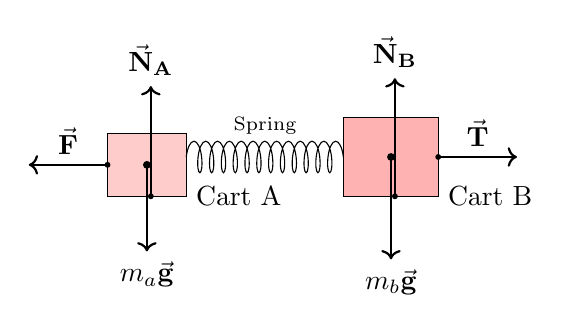
\begin{tikzpicture}

  % Cart A
  \draw[fill=red!20] (0,0) rectangle (1,0.8);
  \node [below, right] at (1,0) {Cart A};

  % Force F
  \draw[<-, thick] (-1,0.4) -- (0,0.4) node[midway, above] {\( \vec{\mathbf{F}} \)};
  \node[circle, fill, inner sep=0.75pt] at (0,0.4) {};

  % Normal reaction
  \draw[->, thick] (0.55,0) -- (0.55,1.4) node[above] {\( \mathbf{\vec{N}_A} \)};
  \node[circle, fill, inner sep=0.75pt] at (0.55,0) {};

  % Gravity
  \draw[->, thick] (0.5,0.4) -- (0.5,-0.7) node[below] {\( m_{a}\vec{\mathbf{g}} \)};
  \node[circle, fill, inner sep=1pt] at (0.5,0.4) {};

  \begin{scope}[shift={(3,0)}]
    % Cart B
    \draw[fill=red!30] (0,0) rectangle (1.2,1);
    \node [below, right] at (1.2,0) {Cart B};

    % Force T
    \draw[->, thick] (1.2,0.5) -- (2.2,0.5) node[midway, above] {\( \vec{\mathbf{T}} \)};
    \node[circle, fill, inner sep=0.75pt] at (1.2,0.5) {};

    % Normal reaction
    \draw[->, thick] (0.65,0) -- (0.65,1.5) node[above] {\( \mathbf{\vec{N}_B} \)};
    \node[circle, fill, inner sep=0.75pt] at (0.65,0) {};

    % Gravity
    \draw[->, thick] (0.6,0.5) -- (0.6,-0.8) node[below] {\( m_{b}\vec{\mathbf{g}} \)};
    \node[circle, fill, inner sep=1pt] at (0.6,0.5) {};
  \end{scope}

  % Spring
  \draw[decoration={aspect=0.3, segment length=1.5mm, amplitude=2mm, coil},decorate] (1,0.5) -- (3,0.5);
  \node at (2,0.9) {\scriptsize{Spring}};

\end{tikzpicture}

\end{document}
